The state estimation described in this thesis will be deployed to two electric \gls{4wd} race cars:
\begin{itemize}
\item a non-autonomous race car which is newly designed and manufactured
\item an autonomous race car which is already existing but repurposed
\end{itemize}
These vehicles will in the following be referred to as \gls{ev} and \gls{dv}, respectively. Note that the \gls{dv} is electric as well but has additional components required for autonomous driving.

\subsection{Sensor Setup}
The vehicles are equipped with a plethora of sensors, which can be used for state estimation. While some sensors like the ones for brake pressure are not relevant, most provide useful information. The relevant sensors are listed in table \ref{tab:sensor}, with the last two columns denoting in which vehicle they are available. In the ideal case, both vehicles would have the all sensors, since working with a homogeneous set of measurements is simpler, but financial and weight considerations mean that only the sensors necessary for the vehicle's use case are available.

\begin{table}
	\newcommand\heading[1]{\textcolor{white}{\textbf{#1}}}
	\renewcommand{\arraystretch}{1.2}
	\sffamily
	\centering
	\begin{tabularx}{\textwidth}{X l c c}
	\rowcolor{black} \heading{Sensor type} & \heading{Measured variables~~~} & \heading{~EV~} & \heading{~DV~} \vspace{2pt} \\
	\Glsdesc{imu}s with gyrometer & $a, \omega$ & \xmark & \xmark \\
	Optical cross-correlation velocity sensor & $v, \beta$ & \xmark &  \\
	Motor speed sensors & $\omega_{motor}$ & \xmark & \xmark \\
	\Glsdesc{gnss} & $p, v$ & \xmark & \xmark \\
	\Glsdesc{gnss} & $\psi$ &  & \xmark \\
	\end{tabularx}
	\caption{Sensor setups for \gls{ev} and \gls{dv}}
	\label{tab:sensor}
\end{table}

The sensor's location in the vehicle are shown in figure \ref{fig:sensor-locations}. The \gls{ev} features three \glspl{imu} with gyrometers: one directly in front of the \gls{cog}, and two situated on the rear left and right. This enables redundancy, since accelerations and rotations in the two-dimensional plane only require two \glspl{imu}. In the \gls{dv}, the front one remains while only a single rear one, denoted by the circle with the missing center, is located directly behind the \gls{cog}. While these sensors react very fast, the signals are rather noisy~\cite[p.~19~ff.]{Biel.2019}.

\begin{figure}
	\centering
	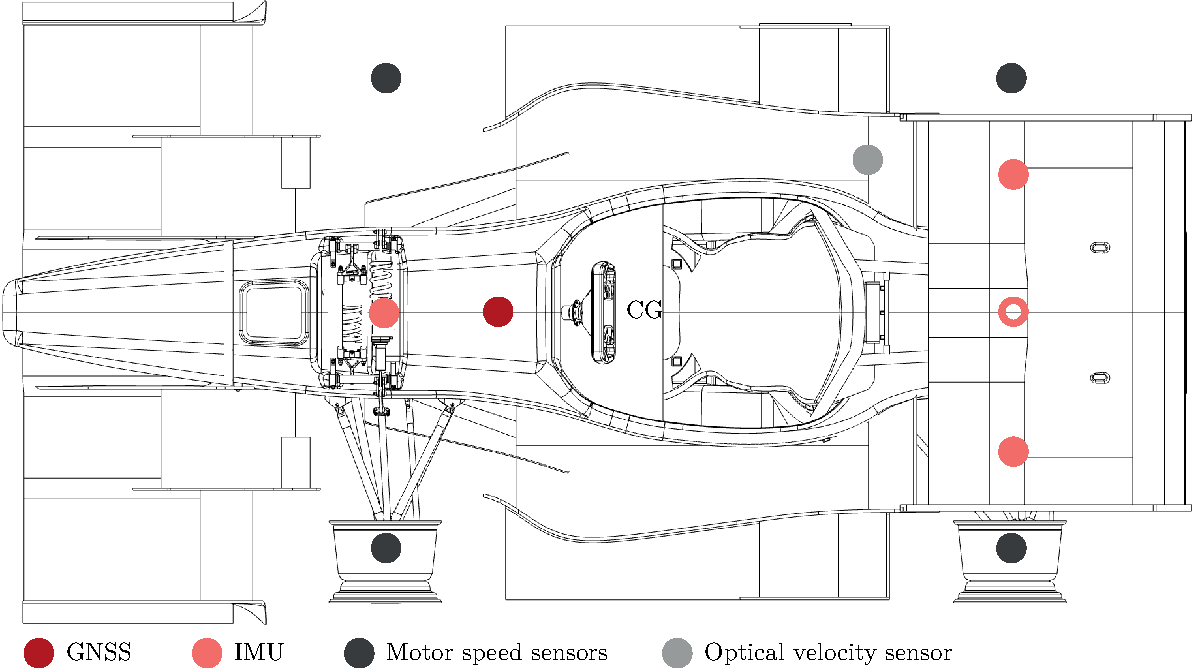
\includegraphics[width=\textwidth]{sensor_locations}%
	\caption{Locations of sensors in vehicle}
	\label{fig:sensor-locations}
\end{figure}

The optical cross-correlation velocity sensor, only available in the \gls{ev}, provides longitudinal and lateral speed measurements, and therefore also measurements of the vehicle sideslip angle. It enables slip-free velocity measurements by correlating photosensor information of the surface over time, which uniquely determines the speed and direction of movement~\cite{Bellof.4241993}. The fact that it is not influenced by slip, as velocity measurements from wheel speeds are, makes it a very valuable addition to the sensor setup. However, it is prone to temporary failures on feature-less surfaces.

The rotary encoders on each of the four motors give individual rotation speed measurements for each of the four wheels. They are available in both vehicles and are assumed to be reliable, since the vehicle will not drive when they fail.

A \gls{gnss} receiver is mounted in the front of both vehicles. Next to position measurements, they provide another source of velocity information. The position accuracy is high in the range of a few centimeters. However, they are slow to react, with over \SI{100}{\milli\second} of delay in some situations~\cite[p.~27]{Biel.2019}. The receiver mounted in the \gls{dv} additionally provides heading information, made possible by the relative position of two separated antennas mounted in the front and rear.

For track and obstacle recognition, the autonomous \gls{dv} is equipped with stereo cameras and lidar sensors. These could be used for optical flow computations to gain more position, attitude and velocity information, but for this design, we rely solely on the sensors described in the previous paragraphs. The estimated state is, however, used to correct lidar measurements.

The key differences between the \gls{ev} and \gls{dv} therefore are as follows:
\begin{itemize}
\item Three \glspl{imu} in \gls{ev} but two \glspl{imu} in \gls{dv}
\item No optical cross-correlation velocity sensor in \gls{dv}
\item No heading information in \gls{ev}
\end{itemize}
The lack of the optical velocity sensor in the \gls{dv} is inconvenient but not fatal, since the state estimation can compensate it.
% TODO plot of velocity from gps, sfii and wheels


\subsection{Computation Hardware}
ECU runs \gls{vdc} with TC, TV, motor request...
The VDC is a tool that helps the driver to exploit the maximum physical potential of the vehicle.
state estimation will be part of \gls{vdc}
In DV vehicle, DV software runs on a separate computer that needs part of state as well
inputs from sensor via CAN at different frequencies to avoid congestion
it is unclear whether sfii will be in DV